\begin{center}
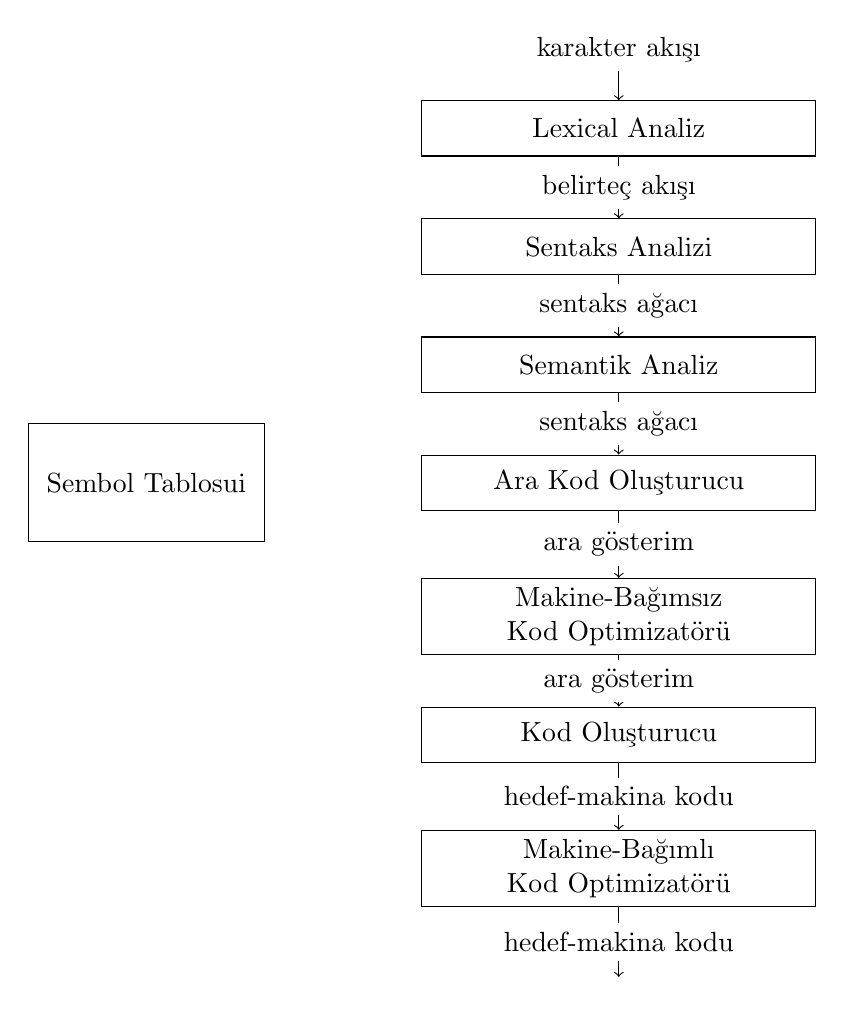
\begin{tikzpicture}[->]
\tikzstyle{rect} = [rectangle, minimum width=5cm, minimum height=0.7cm,text centered, draw=black]
\node (c_str)   {karakter akışı};
\node (lex) [rect, below of=c_str, yshift=-0.01cm] {Lexical Analiz};   
\node (syn) [rect, below of=lex, yshift=-0.5cm] {Sentaks Analizi};   
\node (smn) [rect, below of=syn, yshift=-0.5cm]{Semantik Analiz};   
\node (icode) [rect, below of=smn, yshift=-0.5cm] {Ara Kod Oluşturucu};  
\node (opt) [rect, below of=icode, yshift=-0.7cm,text width=3cm] {Makine-Bağımsız Kod Optimizatörü};  
\node (gen) [rect, below of=opt, yshift=-0.5cm] {Kod Oluşturucu};  
\node (dep_op) [rect, below of=gen, yshift=-0.7cm, text width=3cm,align=center] {Makine-Bağımlı\\Kod Optimizatörü};  
\node (dummy)  [below of=dep_op, yshift=-0.5cm] {};
\node (symbl) [rect, left of=icode, xshift=-5cm, minimum height=1.5cm, minimum width=3cm] {Sembol Tablosui};  

\draw [black](c_str) -- (lex);  
\draw [black](lex) -- node[midway,fill=white] {belirteç akışı} (syn);  
\draw [black](syn) -- node[midway,fill=white] {sentaks ağacı} (smn);  
\draw [black](smn) -- node[midway,fill=white] {sentaks ağacı} (icode);  
\draw [black](icode) -- node[midway,fill=white] {ara gösterim} (opt);  
\draw [black](opt) -- node[midway,fill=white] {ara gösterim} (gen);  
\draw [black](gen) -- node[midway,fill=white] {hedef-makina kodu} (dep_op); 
\draw [black](dep_op) -- node[midway,fill=white] {hedef-makina kodu} (dummy); 

\end{tikzpicture}

Şekil 1.6: Bir derleyicinin aşamaları
\end{center}